\begin{frame}
\frametitle{Pince}
\framesubtitle{Dynamixels 1/2}
\begin{description}
	\item [Caractéristiques]
	\item Moteur électrique de petite taille;
	\item Réducteur pour diminuer la vitesse et augmenter le couple;
	\item  Commande : Largeur impulsion (PWM);
	\item  Temps impulsion : détermine angle à fournir;
	\item  Angle d'ouverture : 0-300°.
\end{description}
\end{frame}

\begin{frame}
\frametitle{Pince}
\framesubtitle{Dynamixels 2/2}
\begin{figure}[!ht]
	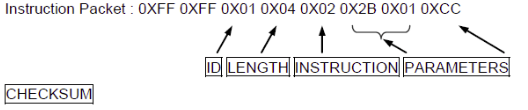
\includegraphics[scale=0.5]{instu.png} 
	\caption{Instruction Packet}
\end{figure}
\end{frame}

\begin{frame}
\frametitle{Pince}
\framesubtitle{Objectifs}
\begin{description}
	\item [Problématique]
	\item Déterminer les tâches;
	\item Pouvoir la contrôler facilement (Software);
	\item Budget.
	\item [Choix]
	\item Design ECAM.
\end{description}
\end{frame}

\begin{frame}
\frametitle{Pince}
\framesubtitle{Contrôle}
\begin{description}
	\item [Comment contrôler les Dynamixels ?]
	\item Libraire Savage;
	\item Arduino.
	\item [Fonctions]
	\item Dynamixel.movespeed(ID,Position,Speed)
	\item Dynamixel.move(ID,Position)
\end{description}
\end{frame}

\begin{frame}
\frametitle{Pince}
\framesubtitle{Catia}
\begin{description}
	\item [En pratique]
	\item Premier test : deux doigts;
	\item Idée : pinces à cheveux;
	\item Deuxième test : 3-2 doigts avec croisement.
\end{description}
\end{frame}
